\chapter{\sys 的总体架构}
\sys 是一个同时支持时序图查询和第一类时序图分析的图处理系统,它由时序图查询和时序图分析两大模块组成。传统的图处理系统通常是基于单一图模型实现的,例如Neo4j是一个基于属性图模型的图数据库,而\sys 将时序属性图、时序RDF图和时序超图三种时序图模型集成到同一系统中。具体来说,\sys 的时序图查询模块同时支持时序RDF图和时序超图两种时序图模型,而时序图分析模块则是基于时序属性图模型实现的。本章将首先介绍系统的总体架构,然后详述系统接口层的实现。

\section{架构概述}
\label{sec:arch}
\sys 的系统架构如图\ref{arch},系统运行在一个由RDMA网络相互连接的集群环境中。
在一个机器数量为$N+2$的集群中,每台机器运行一个服务节点。其中,一个字符串服务器节点用于处理字符串和整型ID之间的转换,一个节点负责处理图的事务化更新和执行系统管理员发起的时序图分析任务(下称分析节点),其余$N$个节点负责处理来自用户的时序RDF图查询请求和时序超图查询请求(下称查询节点)。

\begin{figure}[htb]
\center{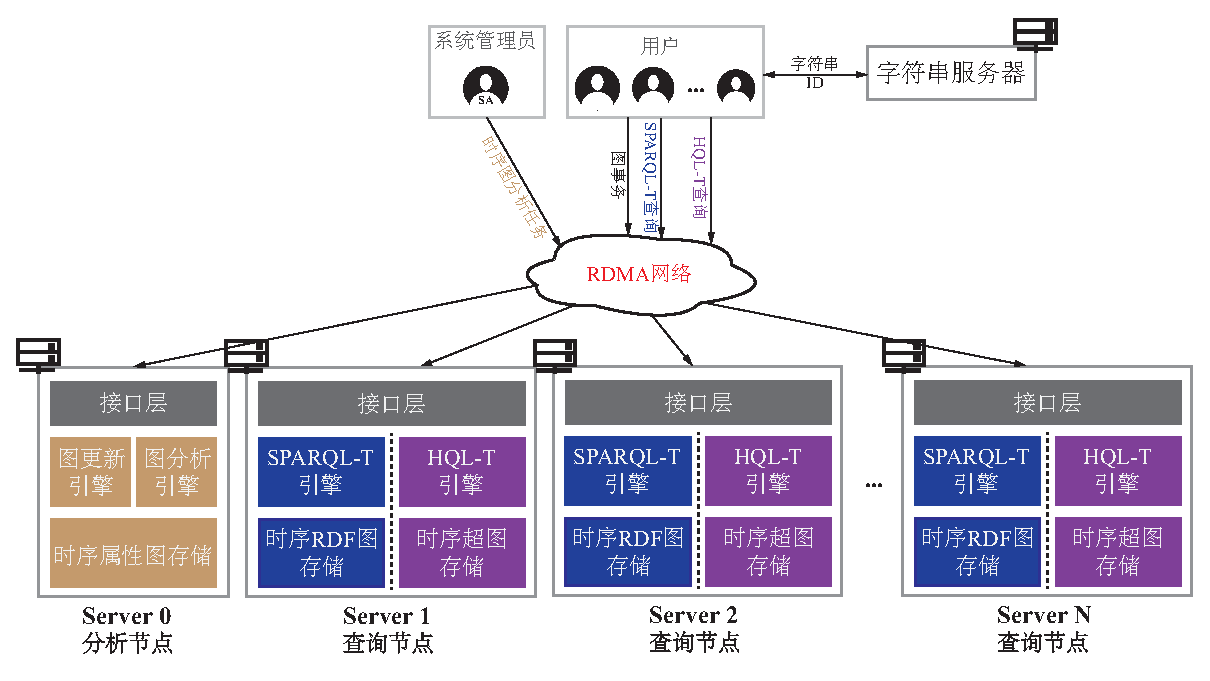
\includegraphics[width=0.87\textwidth]  {figures/arch.eps}} 
\bicaption{\sys 的系统架构}{The architecture of \sys}
\label{arch}
\end{figure}

由于时序RDF图和时序超图都没有标准的查询语言,所以本文设计了系统支持的时序RDF图查询语言和时序超图查询语言,分别命名为SPARQL-T和HQL-T。
在时序RDF图数据集中,时序三元组的主语、谓词和宾语都是字符串,时序超图数据集中的超边名和顶点名也都是字符串。
\sys 在存储时序数据集时,并不直接存储字符串,而是将字符串转化成整型ID进行存储,字符串服务器节点存储了字符串和整型ID之间的映射并负责转换,这一方面减少了系统的内存使用量,另一方面将字符串匹配转换成整型的匹配,加快了匹配速度。用户在发起SPARQL-T和HQL-T查询请求时,会先和字符串服务器节点通信,将查询语句中的字符串转换成整型ID,然后再把它交给系统执行;用户在收到系统返回的查询执行结果时,同样会和字符串服务器节点通信,将查询结果中的ID转回字符串。

\sys 的时序图查询模块采用了去中心化的分布式架构,它采用边割\cite{edgecut}的方式将时序图数据分区存储到$N$个查询节点的内存中以实现水平扩展(章节\S\ref{sec:rdfstore}和\S\ref{sec:hyperstore})。$N$个查询节点是对等的,都能接收和执行来自用户的时序图查询请求,并可以通过RDMA网络实现跨节点的协作,进而提高查询执行的局部性和并行性,提高查询的执行效率。系统的时序图分析模块是单机的,来自用户的图事务请求和来自系统管理员的时序图分析任务都会被转发到分析节点,分别由分析节点的事务处理线程和时序图分析线程来完成。

分析节点和查询节点存储的图数据是相互独立的,查询节点中的时序RDF图和时序超图存储也是相互独立的,图事务请求和时序图分析任务需要读写的是分析节点中的时序属性图存储,SPARQL-T和HQL-T查询请求查询的分别是时序RDF图存储和时序超图存储中的图数据。
由于分析节点需要同时支持图事务和时序图分析,所以时序属性图存储是可读可写的。查询节点只需要支持对时序图数据的检索,时序图数据被加载完毕之后便不会再被更新,因此时序RDF图存储和时序超图存储都是只读的。

除了字符串服务器节点外,系统中的每个节点都由存储层、引擎层和接口层三层组成。存储层负责图数据的存储,并提供访问和更新接口(仅分析节点的存储层提供更新接口)供引擎层使用;引擎层负责图更新、查询和分析任务的执行,它需要使用存储层提供的接口来读写图数据;接口层负责接收来自于用户或系统管理员的请求,将它们解析为系统的内部表示,然后分配给特定节点的引擎层执行。

\section{接口层}
\label{chap:interface}
如\S\ref{sec:arch}所述,接口层负责请求的接收、解析和分配。
接口层由分析节点和查询节点上的若干代理线程和为每个代理线程准备的专用缓冲区来实现。
每个节点的接口层都是对等的,每个代理线程都可以接收和解析来自用户或系统管理员的请求。
节点上的线程分为代理线程和工作线程两种,代理线程位于接口层;工作线程位于引擎层,负责任务的实际执行。
对于分析节点,工作线程又可以分成图事务处理线程和时序图分析处理线程两类;对于查询节点,工作线程负责执行时序图查询任务。
每个线程都有一个专用的缓冲区,线程按照FIFO的顺序从缓冲区中读取请求或结果,本地节点的线程可以直接写缓冲区,远程节点的线程通过单边RDMA Write操作写缓冲区。
代理线程的缓冲区用于接收工作线程的执行结果,工作线程的缓冲区用于接收代理线程或其他工作线程发来的请求。
每个缓冲区被分为$N+1$块,编号为$0, 1, ..., N$,编号为$i (0\leq i \leq N)$的节点只能写缓冲区的第$i$块,这样可以保证不同节点的线程对缓冲区的写不会相互干扰,不需要锁的参与,从而实现节点内和跨节点的高效线程间通信。

\begin{figure}[htb]
\center{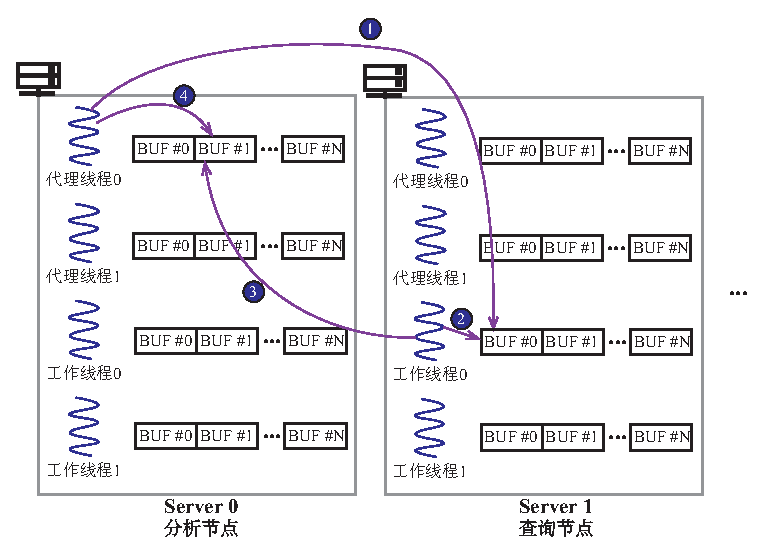
\includegraphics[width=0.7\textwidth]  {figures/interface.eps}} 
\bicaption{线程间的通信流程}{The communication flow between threads}
\label{interface}
\end{figure}

图\ref{interface}演示了线程间的通信流程。
代理线程接收并解析完成请求后,会将请求发送给适当节点的工作线程执行(\ding{182}),方法是使用单边RDMA Write操作写或直接本地写工作线程对应缓冲区中供代理线程所在节点使用的块,然后代理线程会轮询其缓冲区,等待执行结果。
工作线程会轮询其缓冲区,从中读取请求(\ding{183})开始执行。
执行完成后,工作线程会将结果发回代理线程(\ding{184}),方法同样是使用单边RDMA Write操作写或直接本地写代理线程对应缓冲区中供工作线程所在节点使用的块。
此时代理线程就可以读取到请求结果(\ding{185})并返回给用户。

步骤\ding{182}中应该将请求发送给哪个节点的哪个工作线程由以下两个准则决定:
\begin{itemize}
    \item 图事务和时序图分析请求分别会被发送给分析节点的随机图事务工作线程和时序图分析工作线程处理;
    \item 时序图查询请求会被发送给能够使得数据局部性最好的查询节点的随机工作线程执行。虽然RDMA能够高效地实现对远端内存的读取,但它的性能还是落后于对本地内存的读,我们希望查询能够在使得单边RDMA Read操作尽量少、本地内存读尽量多的节点上被处理。
\end{itemize}

\section{本章小结}
本章介绍了\sys 的系统架构。
系统运行在一个由RDMA网络相互连接的集群环境中,集群包含查询节点、分析节点和字符串服务器节点三类节点。
查询节点用于执行来自用户的SPARQL-T和HQL-T查询语句,分析节点用于处理图事务和时序图分析请求,字符串服务器节点用于处理字符串和整型ID之间的转换。
\sys 的时序图查询模块采用了去中心化的分布式架构,而时序图分析模块则是单机的。
每个查询节点和分析节点都由存储层、引擎层和接口层三层组成。存储层负责图数据的存储,引擎层负责图更新、查询和分析任务的执行,接口层负责请求的接收、解析和分配。
本章还对系统的接口层作了详细介绍。接口层由分析节点和查询节点上的若干代理线程和为每个代理线程准备的专用缓冲区来实现,代理线程和工作线程之间可以通过单边RDMA操作实现高效的线程间通信,从而实现高效的请求的分配和执行结果的获取。